%================================================================
\begin{frame}{DataSense Perspectives}

\textbf{Within the STIC Domain}

\begin{itemize}
\item Continuation of the support of collaborative research in the DataSense tasks: both fundamentals and applicative works.
\item Stronger interactions with ComEx and SciLex
  \begin{itemize}
  \item e.g. develop information-theoretic analysis of deep learning
  \item e.g. formal methods meets machine learning, towards safe AI-systems, machine learning for optimizing ontology reasoning...
  \end{itemize}
\item Stronger coordination with DataIA (convergence institute) + Center for Data Science + Optimal Control \& signal communities
  \begin{itemize}
  \item joint calls
  \item (junior) summer schools, software development
  \item Future AI institute (?)
  \end{itemize}
\end{itemize}
\end{frame}


%================================================================
\begin{frame}{DataSense Perspectives}

\textbf{Beyond STIC}: given the maturity of the domain, time to open to new communities

\begin{itemize}
\item Open Digicosme to new labs (e.g. INRA maIAGE; INRA mia )
\item E-science: have more common projects with  other departments
  \begin{itemize}
  \item Life science
  \item physics
  \item (?) SHS
  \item Maths, theoretical physics
  \end{itemize}
\end{itemize}

\begin{center}
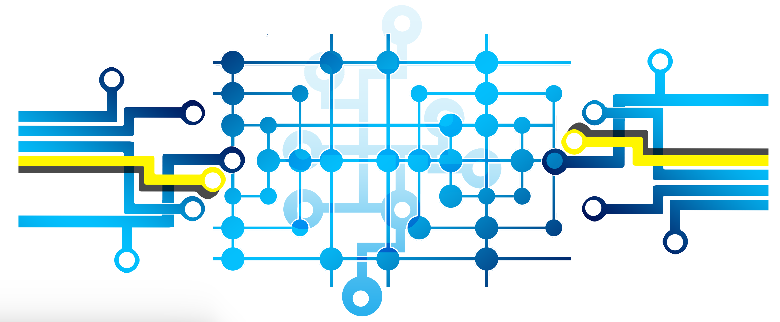
\includegraphics[width=.75\linewidth]{Images/datasense.png}
\end{center}

\end{frame}

%================================================================
\begin{frame}[plain]{}

  \vfill
  \begin{center}
    \huge THANK YOU!
  \end{center}
  \vfill

\end{frame}

%%% Local Variables: 
%%% mode: latex
%%% coding: utf-8-unix
%%% ispell-local-dictionary: "english"
%%% TeX-master: "datasense-2016.tex"
%%% fill-column: 9999
%%% End: 
